\begin{center}

  \begin{tabular}{rp{6cm}lp{12cm}}%{rl}

  % after \\: \hline or \cline{col1-col2} \cline{col3-col4} ...

  论文地址:& \href{https://arxiv.org/abs/1912.11615}{https://arxiv.org/abs/1912.11615} \\

  %源码:& \href{xxx}{xxx} \\

%  slides:& \href{http://yunshengb.com/wp-content/uploads/2017/03/nips_2018_r2l_workshop_talk.pdf}{{\footnotesize Convolutional Set Matching for Graph Similarity}}\\

  关键词:& \textbf{Metric learning, Graph similarity, GNN} \\

  写于:& \date{2020-10-17}

  \end{tabular}

\end{center}

该论文\cite{ma2020deep}对近年来使用深度学习/GNN计算图相似性的方法进行了一个较为全面的总结,对每种方法进行了一个简要的介绍,描述了图相似性常用的数据集和评估方法,并对图相似性计算的应用及该领域内现存的挑战和难点进行了全面的概括。

图的相似性计算是一种metric learning,学习如何度量两个对象之间的距离。图之间的相似性可以用一个0到1之间的小数表示,但是关键在于如何学习到这样的一个similarity score。

\begin{figure}[h]
	\centering
	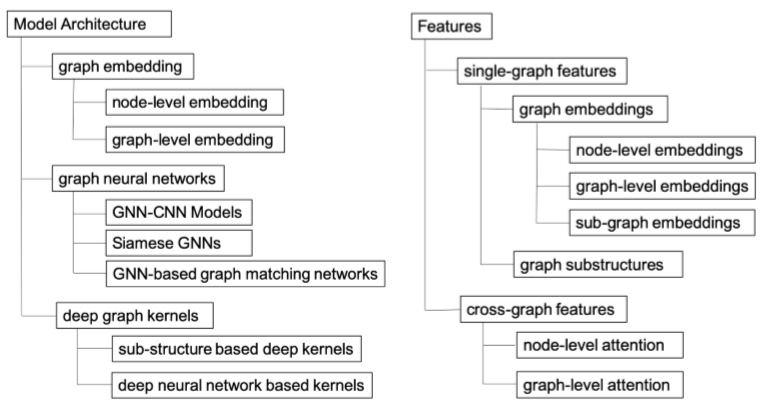
\includegraphics[width=.75\textwidth]{pics/taxonomy_dgs.PNG}
	\caption{Taxonomy of DGS}
	\label{fig:taxonomy_dgs}
\end{figure}

如Fig.\ref{fig:taxonomy_dgs}所示,可以按照模型结构和单/多图的特征来进行分类。按照模型结构,论文中对现有的深度图相似性学习方法主要分为以下三类:
\begin{itemize}
	\item graph-embedding based:使用通过graph embedding方法得到的结点/图表征来计算相似度,如graph2vec,node2vec等
	\item graph neural networks based:在图相似的任务中,以end-to-end的方式使用GNN来学习相似度,如GSimCNN,SimGNN,Siamese GCN等
	\item deep graph kernel based:通过学习核函数来计算同之间的相似性,如Deep graph kernels,Deep divergence graph kernel等
\end{itemize}

论文中对图相似的应用归纳如下:
\begin{itemize}
	\item 在生物信息领域内的应用。例如学习化学元素、分子、化合物等的相似性,研究它们之间的相互作用
	\item 在脑科学中,检测脑网络结构的相似性,分析脑网络的功能。可以指示脑网络功能的正常与否
	\item 计算机安全。可以用来对代码进行分析,
	\item 在计算机视觉中的应用,用于视频序列中动作行为的识别
\end{itemize}

论文中对图相似性的挑战归纳如下:
\begin{itemize}
	\item 在复杂的图数据上的相似性计算。如有向图、动态图/流图、
	\item 解释学习到的结果。
	\item 小样本学习(few-shot learning)。当每一类只有少量数据时如何学习相应的分类器
\end{itemize}

有几个注意的点:
\begin{itemize}
	\item 一个图与自身的相似性要大于等于任何与其他图的相似性,即$s_{ii} >= s_{ij}$
	\item 数据的对齐直觉上是将不同空间/分布的数据放在同一个空间/分布中,但依然能够保持它们原有的某些性质(包括intar,inter的性质)
	\item 在相似性计算时利用结点/边的特征
	\item 由于脑网络的特殊性,脑网络中的相似性更应该是一个子图学习的问题
\end{itemize}
%\paragraph{xxx思路}

%\paragraph{方法解决的问题/优势}
%\begin{itemize}

%	\item 

%\end{itemize}



%\paragraph{方法的局限性/未来方向}

%\begin{itemize}

%	\item 

%\end{itemize}




